\documentclass[11pt]{article}\usepackage[]{graphicx}\usepackage[]{color}
%% maxwidth is the original width if it is less than linewidth
%% otherwise use linewidth (to make sure the graphics do not exceed the margin)
\makeatletter
\def\maxwidth{ %
  \ifdim\Gin@nat@width>\linewidth
    \linewidth
  \else
    \Gin@nat@width
  \fi
}
\makeatother

\definecolor{fgcolor}{rgb}{0, 0, 0}
\newcommand{\hlnum}[1]{\textcolor[rgb]{0,0,0}{#1}}%
\newcommand{\hlstr}[1]{\textcolor[rgb]{0,0,0}{#1}}%
\newcommand{\hlcom}[1]{\textcolor[rgb]{0.4,0.4,0.4}{\textit{#1}}}%
\newcommand{\hlopt}[1]{\textcolor[rgb]{0,0,0}{\textbf{#1}}}%
\newcommand{\hlstd}[1]{\textcolor[rgb]{0,0,0}{#1}}%
\newcommand{\hlkwa}[1]{\textcolor[rgb]{0,0,0}{\textbf{#1}}}%
\newcommand{\hlkwb}[1]{\textcolor[rgb]{0,0,0}{\textbf{#1}}}%
\newcommand{\hlkwc}[1]{\textcolor[rgb]{0,0,0}{\textbf{#1}}}%
\newcommand{\hlkwd}[1]{\textcolor[rgb]{0,0,0}{\textbf{#1}}}%
\let\hlipl\hlkwb

\usepackage{framed}
\makeatletter
\newenvironment{kframe}{%
 \def\at@end@of@kframe{}%
 \ifinner\ifhmode%
  \def\at@end@of@kframe{\end{minipage}}%
  \begin{minipage}{\columnwidth}%
 \fi\fi%
 \def\FrameCommand##1{\hskip\@totalleftmargin \hskip-\fboxsep
 \colorbox{shadecolor}{##1}\hskip-\fboxsep
     % There is no \\@totalrightmargin, so:
     \hskip-\linewidth \hskip-\@totalleftmargin \hskip\columnwidth}%
 \MakeFramed {\advance\hsize-\width
   \@totalleftmargin\z@ \linewidth\hsize
   \@setminipage}}%
 {\par\unskip\endMakeFramed%
 \at@end@of@kframe}
\makeatother

\definecolor{shadecolor}{rgb}{.97, .97, .97}
\definecolor{messagecolor}{rgb}{0, 0, 0}
\definecolor{warningcolor}{rgb}{1, 0, 1}
\definecolor{errorcolor}{rgb}{1, 0, 0}
\newenvironment{knitrout}{}{} % an empty environment to be redefined in TeX

\usepackage{alltt}
\usepackage{fullpage,graphicx,float,amsmath,enumitem,hyperref}
\setlist{parsep=5.5pt}
\setlength{\parindent}{0pt}
\setlength{\parskip}{\baselineskip}

\usepackage{fancyhdr}
\pagestyle{fancy}
\lhead{Draft}
\rhead{Time Series Project}
\setlength{\headheight}{18pt}
\setlength{\headsep}{2pt}

\title{ARCH, GARCH, and Volatility}
\author{Andrea}
\date{\today}
\IfFileExists{upquote.sty}{\usepackage{upquote}}{}
\begin{document}
\maketitle






An important results from Extreme Value Theory (EVT) concerns tails of distributions. To quantify the probability of losing a certain value of money above a threshold, it can be shown that the distribution of values above the threshold converges to the generalized PARETO distribution if the threshold is set high enough, known as the Peak Over Threshold method. The pdf of a generalized PARETO distribution is:

f(x) = $\frac{1}{\sigma}(1 + \zeta\frac{(x-\mu)}{\sigma})^{-\frac{1}{\zeta} + 1}$

with $\mu \in \Re; \sigma \in + \Re; \zeta \in \Re$.

Comparatively, the PARETO distribution are parameterized in Casella and Berger is:

f(x) = $\frac{\beta\alpha^{\beta}}{x^{\beta + 1}}$

with $\alpha, \beta \> 0$ and $\alpha < x <$ \infty

Note that there are four different Types of PARETO distributions in addition to the Lomax parameterization (Wikipedia).

This is compared to the more familiar PARETO distribution (and give curves)

\begin{knitrout}\footnotesize
\definecolor{shadecolor}{rgb}{1, 1, 1}\color{fgcolor}

{\centering 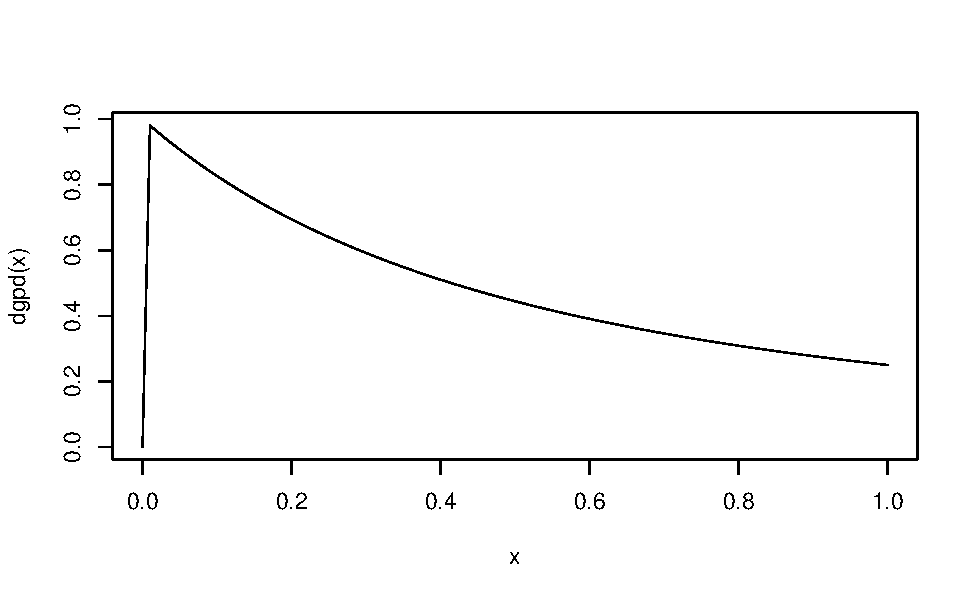
\includegraphics[width=\maxwidth]{figure/pareto-1} 

}


\begin{kframe}

{\ttfamily\noindent\bfseries\color{errorcolor}{Error in dgamma(x): argument "{}shape"{} is missing, with no default}}\end{kframe}
\end{knitrout}


\end{document}
